\documentclass[10pt]{article}
\usepackage{../../local}
\urlstyle{same}

\newcommand{\classcode}{EE120}
\newcommand{\classname}{Signals and Systems}
\renewcommand{\maketitle}{%
\hrule height4pt
\large{Eric Du \hfill \classcode}
\newline
\large{HW 07} \Large{\hfill \classname \hfill} \large{\today}
\hrule height4pt \vskip .7em
\small{Header styling inspired by CS 70: \url{https://www.eecs70.org/}}
\normalsize
}
\linespread{1.1}
\begin{document}
	\maketitle
	\section*{Collaborators}
	I worked with the following people on this assignment:
	\begin{itemize}
		\item Teja Nivarthi: 3036508567
		\item Nikhil Maserang: 3036978230
	\end{itemize}
	\pagebreak
	\section*{Problem 1}
	Consider a discrete-time signal \( x: \Z \to \R \) having the following properties:
	\begin{itemize}
		\item \( x[n + 4l] = x[n], \ \forall l, n \in \Z\)
		\item \( \sum_{n = -1}^{2}x[n] = 2 \) 
		\item \( \sum_{n=-1}^{2} (-1)^{n}x[n] = 4 \) 
		\item \( \sum_{n=-1}^{2} x[n] \cos\left[ \frac{\pi}{2}n \right] = \sum_{n=-1}^{2} x[n] 
			\sin\left[ \frac{\pi}{2}n \right] = 0\)
	\end{itemize}
	\begin{enumerate}[label=\alph*)]
		\item Determine the complex exponential Fourier series coefficients \( X_{-1}, X_0, X_1 \) and 
			\( X_2 \) for the signal \( x \). From the coefficients, determine and provide a well-labeled
			plot for the signal \( x \). 

			\begin{solution}
				Recall the formula for calculating the Fourier coefficients:
				\[
					X_k = \frac{1}{N_0}\sum_{n=0}^{N_0-1} x[n] e^{-j k \omega_0 n} \quad k = 0, 1, 2, \dots
				\]  
				From \( x[n] = x[n + 4l] \) we know that \( x[n] = x[n + 4] \), implying that 
				\( N_0 = 4 \). Thus, \( \omega_0 = \frac{2\pi}{4} = \frac{\pi}{2} \). Now, from the 4th condition, we 
				can identify:
				\begin{align*}
					\frac{1}{4}\left(\sum_{n=-1}^{2} x[n] \cos\left[ \frac{\pi}{2}n \right] + 
					i \sum_{n=-1}^{2} x[n] \sin\left[ \frac{\pi}{2}n \right]\right) = \frac{1}{4}\sum_{n=-1}^{2} x[n]
					e^{i \frac{2\pi}{4} n} = X_{-1} = 0
				\end{align*}
				Same goes for \( X_1 \) (so we have \( X_{-1} = X_1 = 0 \)), 
				since the formula is the same up to a minus sign. For \( X_0 \), we have:
				\[
					X_0 = \frac{1}{4}\sum_{n=-1}^{2} x[n] = \frac{1}{2}
				\] 
				and for \( X_2 \):
				\begin{align*}
					X_2 &=\frac{1}{4} \sum_{n=-1}^{2} e^{-i \frac{2\pi}{4} (2n)}\\
						&= \frac{1}{4}\sum_{n=-1}^{2} x[n] e^{-i \pi n} \\
						&=\frac{1}{4} \sum_{n=-1}^{2} (-1)^{n}x[n] = 1
				\end{align*}
				and that completes all of them. Now, we use the synthesis equation to recover \( x[n] \):
				\[
					x[n] = \sum_{n=-1}^{2} X_k e^{j k \omega_0 n}
				\] 
				Notice that since \( X_{-1} = X_1 = 0 \), then only \( k = 0, 2 \) terms are nonzero. Therefore, 
				we can write:
				\[
					x[n] = \frac{1}{2} + e^{j \pi n} = \frac{1}{2} + (-1)^{n}
				\] 
				Crunching the numbers, this gives us:
				\begin{align*}
					x[-1] &= -\frac{1}{2} \\
					x[0] &= \frac{3}{2} \\
					x[1] &=  -\frac{1}{2} \\
					x[2] &= \frac{3}{2} 
				\end{align*}
				As for a plot, this is quite easy:
				\begin{center}
					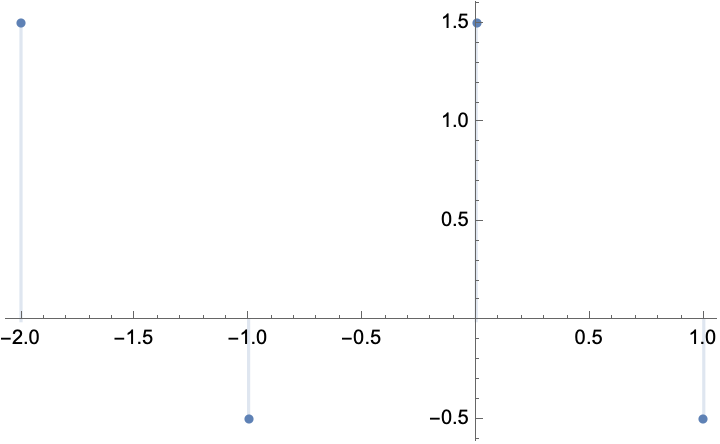
\includegraphics[scale=0.8]{q1a.png}
				\end{center}
			\end{solution}
		\item Based on your results from part (a), determine the fundamental period \( p \) and 
			fundamental frequency \( \omega_0 \) of the signal \( x \). Express \( x \) in terms of 
			its DTFS coefficients and complex exponentials of appropriate frequencies, and identify 
			each coefficient and its corresponding harmonic frequency. 

			\begin{solution}
				We actually see that even though \( x[n] = x[n + 4] \), this is not the fundamental period
				since \( x[n]  \) actually only oscillates over 2 values. Therefore, the fundamental period 
				is 2, and we have \( N_0 = p =  2 \) so \( \omega_0 = \frac{2\pi}{T} = \pi \). Recalculating 
				\( X_k \):
				\[
					X_k =  \frac{1}{2}(x[0] + x[1] e^{- j \pi k} )
				\]
				This implies that \( X_0 = \frac{1}{2} \) and \( X_1 = 1 \). Now, recalculating \( x[n] \), 
				we have:
				\[
					x[n] = X_0 + X_1e^{ j \pi n} = \frac{1}{2} + (-1)^{n}
				\] 
				this matches exactly what we got from part (a). As for identifying the coefficients, we have 
				\( X_0 \) corresponds to \( \omega = 0 \), and \( X_1 \) corresponds to \( \omega = \pi \). These 
				coefficients repeat (since \( x \) is periodic), so this means that the even numbered \( X_k \) 
				implicitly correspond to \( \omega = 0 \), and the odd ones implicitly correspond to \( \omega = \pi \).
			\end{solution}
	\end{enumerate}
	\pagebreak
	\section*{Problem 2} 
	Consider a periodic, discrete-time signal \( x: \Z \to \R \) having the discrete-time Fourier series
	(DTFS) expansion
	\[
		x[n] = \sum_{k = \mean p} X_k e^{j k \omega_0 n }
	\] 
	where \( \omega_0 \) denotes the fundamental frequency of the signal; if \( p \) is the period of \( x \), then 
	\( \omega_0 = 2\pi / p\). 

	Suppose \( x \) is the input signal applied to a linear time-invariant (LTI) system characterized by the impulse 
	response \( h: \Z \to \R \) and corresponding frequency response \( H \), where 
	\[
		H(e^{i \omega}) = \sum_{n=-\infty}^{\infty} h[n] e^{-j \omega n}, \quad \forall \omega
	\] 
	Let \( y \) be the corresponding output signal.
	\begin{enumerate}[label=\alph*)]
		\item Prove that the output signal \( y \) is periodic; that is, show that if  \( x[n + p] = x[n] \), then 
			\( y[n + p] = y[n] \). 

			\begin{solution}
				We know that \( y[n] = x[n] * h[n] \), then by the symmetry of the convolution, we also 
				have  \( y[n] = h[n] * x[n] \). Therefore, for \( y[n + p] \), we have:
				\[
					y[n + p] = \sum_{k=-\infty}^{\infty} h[k] x[n + p - k]
				\] 
				but since \( x[n] = x[n + p] \), then we know \( x[n + p - k] = x[n - k] \), hence:
				\[
					y[n + p] = \sum_{k=-\infty}^{\infty} h[k] x[n - k] = h[n] * x[n] = y[n]
				\] 
				as desired. 
			\end{solution}
			\item Let the DTFS expansion of the output signal \( y \) be
			\[
				y[n] = \sum_{k = \mean p} Y_k e^{j k \omega_0 n }
			\] 
			\begin{enumerate}[label=\roman*)]
				\item Express the output-signal DTFS coefficients \( Y_k \) in terms of the input signal DTFS
					\( X_k \) and the frequency response \( H \).

					\begin{solution}
						We know that based on convolution properties:
						\[
						Y_k = X_k H_k
						\] 
						where \( H_k \) represents \( H(e^{i \omega}) \) sampled at the point \( \omega = k \omega_0 \).
						Therefore, we write:
						\[
						Y_k = X_k H(e^{i k \omega_0})
						\] 
						% ask about why this is even valid to begin with 
					\end{solution}
				\item Suppose the impulse response of the LTI system is given by 
					\( h[n] = \delta[n -  n_0] \), where \( n_0 \in \Z \). Explicitly determine the output-signal 
					DTFS coefficients \( Y_k \) in terms of the input-signal DTFS coefficients
					\( X_k \).

					\begin{solution}
						Based on the given \( h[n] \), then we can determine:
						\[
							H(e^{j \omega}) = \sum_{n=-\infty}^{\infty} h[n] e^{- j \omega n} = 
							\sum_{n=-\infty}^{\infty} \delta[n - n_0] e^{- j \omega n} = e^{- j \omega n_0}
						\] 
						Now, using the previous part, we get:
						\[
						Y_k = X_k H(e^{j k \omega_0}) = X_k e^{-j \omega k n_0}
						\] 
					\end{solution}
			\end{enumerate}
	\end{enumerate}
	\pagebreak
	\section*{Problem 3}
	A bandlimited continuous-time signal \( x \) has the triangular spectrum shown below:
	\begin{center}
		\begin{tikzpicture}[scale=1.5]
			\draw[-stealth] (-2, 0) -- (2, 0) node[above] {\( \omega \) };
			\draw[-stealth] (0, 0) -- (0, 1.5) node[right] {\( X(\omega) \) };
			\draw[blue, semithick](-1, 0) -- (0, 1) -- (1, 0);
			\draw (-0.05, 1) node[left] {1}-- (0.05, 1);
			\draw (-1, 0.05) -- (-1, -0.05) node[below] {\( -A \) };
			\draw (1, 0.05) -- (1, -0.05) node[below] {\(+ A \) };
		\end{tikzpicture}
	\end{center}
	The following diagram shows an amplitude modulation-demodulation scheme to communicate signal \( x \) to 
	a receiver. In this problem, you'll explore the effects of frequency mismatch between the transmitter and 
	receiver carriers \( q_T \) and \( q_R \) respectively. 
	\begin{center}
		\begin{circuitikz}
    \draw[thick,->] (-1.5,0) node[left]{$x(t)$} -- (-0.4,0);
    \draw (0,0) to (0,0) node[mixer,scale=0.75] (mix){} 
    (mix) to[short] (1.75,0) to (1.75,1) node[bareantenna,scale=0.75]{};
    \node at (1,0.25) (r) {$r(t)$};
    \draw[thick,->] (0,-1) node[below] {$q_T(t) = \cos(\omega_0t)$} -- (0,-0.4);
    \begin{scope}[xscale=-1,yscale=1]
        \draw[thick,<-] (-6.5,0) node[right]{$y(t)$} -- (-5.4,0);
        \draw (-5,0) to (-5,0) node[mixer,scale=0.75] (mix){};
        \draw[<-]
        (mix) to[short] (-3.25,0);
        \draw (-3.25,0) to (-3.25,1) node[bareantenna,scale=0.75]{};
        \node at (-4,0.25) (r) {$r(t)$};
        \draw[thick,->] (-5,-1) node[below] {$q_R(t) = \cos(\omega_1t)$} -- (-5,-0.4);
    \end{scope}
\end{circuitikz}
	\end{center}
	In particular, assume that 
	\[
	0 < \epsilon \ll A < \omega_0 = \omega_1 + \epsilon
	\] 
	\begin{enumerate}[label=\alph*)]
		\item Determine reasonably simple expressions for the signals \( r \) and \( y \). You may find the following 
			trigonometric identity useful:
			\[
				\cos \alpha \cos \beta = \frac{1}{2}[\cos(\alpha + \beta) + \cos(\alpha - \beta)]
			\] 

			\begin{solution}
				This is an AM modulation scheme, so we have:
				\[
				r(t) = x(t) q_T(t) = x(t) \cos(\omega_0 t)
				\] 
				Then, we since we multiply by \( q_R(t) \), then we have:
				\[
				y(t) = x(t) q_T(t) q_R(t) = x(t) \cos(\omega_0 t) \cos(\omega_1 t)
				= \frac{x(t)}{2}[\cos((\omega_0 + \omega_1)t) + \cos((\omega_0 - \omega_1) t) 
				\] 
				to find \( x(t) \), we have to take the inverse Fourier transform of \( X(\omega) \). The functional 
				form of \( X(\omega) \) is:
				\[
				X(\omega) = \begin{cases}
					\frac{\omega}{A} + 1 & \omega < 0\\
					-\frac{\omega}{A} + 1 & \omega > 0
				\end{cases}
				\] 
				Performing the Fourier transform, we ultimately get:
				\[
				x(t) = \frac{1 - \cos(At)}{A \pi t^2}
				\] 
				So fnally, we have:
				\begin{align*}
					r(t) &= \frac{1 - \cos(At)}{A \pi t^2} \cos (\omega_0 t)\\
					y(t) &= 
					\frac{1 - \cos(At)}{2 A \pi t^2}[\cos((\omega_0 + \omega_1)t) + \cos((\omega_0 - \omega_1)t) ]
				\end{align*}
			\end{solution}
		\item Provide well-labeled plots of \( R(\omega)  \) and \( Y(\omega) \), the spectra of the signals \( r \) 
			and \( y \), respectively.

			\begin{solution}
				For \( R(\omega) \), we take the Fourier transform, and from lecture we know that:
				\[
					R(\omega) = \frac{1}{2}[X(\omega - \omega_0) + X(\omega + \omega_0)]
				\] 
				so this will look like two triangles that are symmetric about \( \omega = 0 \). A plot is given 
				below, plotted in Mathematica using \( A = 2, \omega_0 = 3 \):
				\begin{center}
					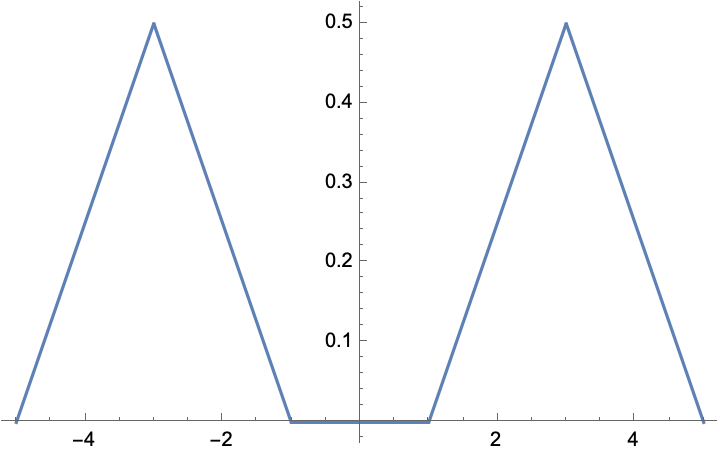
\includegraphics[scale=0.8]{q3c1.png}
				\end{center}
				For \( Y(\omega) \), we can use the same argument, giving us:
				\[
				Y(\omega) = \frac{1}{2}\left[ X(\omega - (\omega_1 + \omega_0))+ X(\omega + (\omega_1 + \omega_0))
				+ X(\omega - (\omega_1 - \omega_0)) + X(\omega + (\omega_1 - \omega_0))\right] 
				\] 
				For the same parameters above and  \( \omega_1 = 2 \), the plot looks like this:
				\begin{center}
					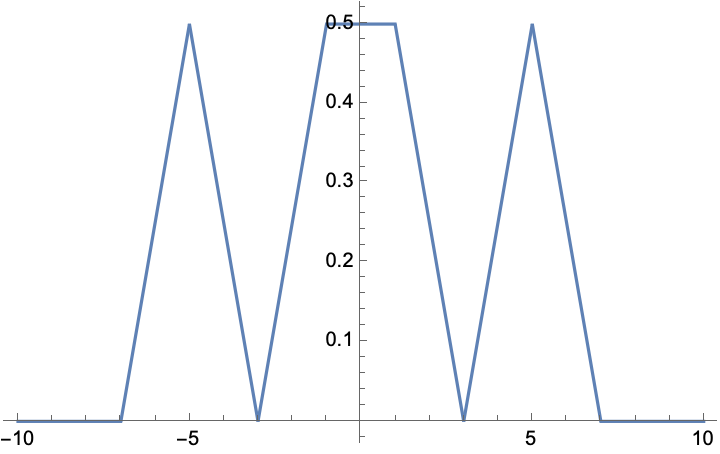
\includegraphics[scale=0.8]{q3c2.png}
				\end{center}
			\end{solution}
		\item Explain why the information-bearing signal \( x \) is irrecoverable, even if we send the signal \( y \) 
			through an ideal low-pass filter. 

			\begin{solution}
				An ideal low-pass filter will filter out all signals above a certain frequency \( \omega = \omega_c \).
				However, we see that \( Y(\omega) \) has overlapping spikes, meaning that we won't be able 
				to discern our signal \( x(t)  \) out clearly.  
			\end{solution}
	\end{enumerate}
	\pagebreak
	\section*{Problem 4} 
	Consider an LTI system with frequency response as follows
	\[
	H(e^{j \omega}) = \frac{e^{- j \omega} - a}{1 - ae^{- j \omega}}
	\] 
	where \( a \) is a real number such that \( |a| < 1 \).
	\begin{enumerate}[label=\alph*)]
		\item Show that \( |H(e^{j \omega})| = 1 \) at all frequencies. What kind of filter is this?

			\begin{solution}
				We just do the algebra:
				\[
				|H(e^{j\omega})|^2 = \frac{e^{- j \omega} - a}{1 - ae^{-j \omega}}\frac{e^{j \omega} - a}{1 - 
				ae^{j \omega}} = \frac{1 - ae^{- j \omega} - ae^{j \omega} + a^2}{1 - ae^{j \omega} - ae^{- j \omega}
			+ a^2} = 1 \implies |H(e^{j \omega})| = 1
				\] 
				Because \( M(\omega) = 1 \) for all \( \omega \), this is considered an all-pass filter. 
			\end{solution}
		\item Derive an expression for the phase \( \angle H(e^{j \omega}) \).

			\begin{solution}
				The algebra in this question is relatively long, so I'm going to skip most of it. Firstly, we
				 know that
				 \[
				 \angle H(e^{j \omega}) = \tan^{-1}\left( \frac{\Im(H)}{\Re(H)} \right) 
				 \] 
				 So to find these two expressions, we first express \( H \) in terms of its real and 
				 imaginary parts:
				 \[
				 H(e^{j \omega}) = \frac{\cos(\omega) - i \sin(\omega) - a}{1 - a(\cos \omega - i \sin(\omega)}
				 = \frac{\cos(\omega) - a - i \sin(\omega)}{1 - a \cos(\omega) - ia \sin(\omega)}
				 \] 
				 Now we multiply to make the denominator a real quantity:
				 \[
				 \frac{(\cos (\omega) - a - i \sin(\omega))(1 - a\cos(\omega) + ia \sin(\omega)}{(1 + a \cos(\omega))^2
				 + a^2 \sin^2 (\omega)}
				 \] 
				 From here, we expand the numerator, and collect the real and imaginary part. Because they're being 
				 divided together, the denominator doesn't actually matter here. Therefore, our 
				 final expression (again, skipping the algebra because I can't be bothered to type 
				 it out): 
				 \[
				 \angle H(e^{j \omega}) = \tan^{-1}\left[ \frac{a \sin (\omega) \cos (\omega) - a^2\sin(\omega)
				 - \sin(\omega) + \cos(\omega)}{\cos(\omega) - a \cos^2(\omega) - a + a^2\sin(\omega) 
			 \cos(\omega) + a \sin^2(\omega)} \right] 
				 \] 
				 yeah. Not a nice expression, but oh well. 
			\end{solution}
		\item Take \( a = \frac{1}{\sqrt{3} } \) and determine the output \( y[n] \) for the input
			\[
				x[n] = \cos\left[ \frac{\pi}{6}n \right]  + \cos[\pi n]
			\] 

			\begin{solution}
				Following what I saw on Ed, we write \( x[n] \) in terms of exponentials:
				\[
					x[n] = \frac{1}{2}(e^{i \frac{\pi}{6}n} + e^{- i \frac{\pi}{6}n} + e^{i \pi n } + e^{- i \pi n})
				\] 
				Now, we use the fact that given a signal \( x[n] = Ae^{i \omega n} \), then the output 
				\( y[n] = H(\omega) Ae^{i \omega n} \). Using this fact, we get:
				\[
					y[n] = \frac{1}{2}\left( H\left( \frac{\pi}{6} \right) e^{i \frac{\pi}{6}n}
					+ H\left( -\frac{\pi}{6} \right) e^{- i \frac{\pi}{6}n} + H(\pi) e^{i \pi n} + 
				H(-\pi) e^{-i \pi n}\right) 
				\] 
				I'm not convinced that plugging in the values for \( H \) would give you a much nicer 
				expression so I'm going to leave it at this.
			\end{solution}
		\item Write a difference equation that implements an LTI system with the frequency response 
			above. 

			\begin{solution}
				Based on the previous problems we've had, we know that for an LCCDE equation of the form:
				\[
					a_0y[n] + \cdots + a_ky[n - k] = b_0x[n] + \cdots + b_l x[n - l]
				\] 
				the frequency response \( H(\omega) \) is given by:
				\[
				H(\omega) = \frac{\sum_{m=0}^{k} b_m e^{-i \omega m}}{\sum_{n=0}^{k} a_n e^{-i \omega n}}
				\] 
				Based on our \( H(\omega)  \) we have above, this implies that \( b_0 = -1, b_1 = 1 \) and 
				\( a_0 = 1, a_1 = -a \). Therefore, we have:
				\[
					y[n] - ay[n - 1] = -x[n] + x[n - 1]
				\] 
			\end{solution}
	\end{enumerate}
	\pagebreak
	\section*{Problem 5}
	The impulse response of a real, discrete time FIR filter A is described by
	\[
		a[n] = a_0\delta[n] + a_1\delta[n - 1] + \cdots + a_N \delta[n - N] \quad \text{where \( N \in 
		\{1, 2, 3, \dots\} \)}
	\] 
	\begin{enumerate}[label=\alph*)]
		\item Show that the frequency response \( A(e^{j \omega}) \) of the filter is a polynomial, in terms of 
			\( e^{- j \omega} \), whose coefficients have a simple relationship with the impulse response 
			value \( a_0, \dots, a_N \). 

			\begin{solution}
				Since the impulse response is given by replacing \( x[n]  \) with \( \delta[n] \), we can just flip 
				it back to get the filter equation:
				\[
					\mathcal A [n] = a_0 x[n] + a_1 x[n - 1] + \cdots + a_N x[n - N]
				\] 
				Now, using the same approach as question 4d, we can use the expression:
				\[
					H(\omega) = \frac{\sum_{m=0}^{k} b_m e^{-i \omega m}}{\sum_{n=0}^{k} a_n e^{-i \omega n}}
				\] 
				to get our value for \( A(e^{j \omega}) \). Here, this comes out to be:
				\[
				A(e^{j \omega}) = \sum_{m=0}^{N} a_m e^{- j \omega m}
				\] 
				this is a polynomial in terms of \( e^{- j \omega} \), whose coefficients are exactly 
				the impulse response values \( a_0, \dots, a_N \). 
			\end{solution}
		\item Suppose the filter \( \mathcal A \) is plaed in a cascade (series) interconection with another 
			discrete-time FIR filter \( \mathcal B \) whose impulse response is describd by 
			\[
				b[n]= b_0\delta[n] + b_1\delta[n-1] + \cdots + b_M \delta[n - M], \quad \text{where \( M \in 
				\{ 1, 2, 3, \dots\} \)}
			\] 
			The cascade structure which we call \( \mathcal C \) is shown in the figure below.
			%diagram
			Let  \( c[n] \) denote the impulse response of hte cascade interconnection.
			\begin{enumerate}[label=\alph*)]
				\item Expression \( c[n] \) in terms of \( a[n] \) and \( b[n] \). 

					\begin{solution}
						Because the systems are being placed in series with each other, then we know that 
						\[
							c[n] = a[n] * b[n]
						\] 
					\end{solution}
				\item Express the frequency response \( C(e^{j \omega}) \) of the system \( \mathcal C \) in terms 
					of the frequency responses \( A(e^{j \omega}) \) and \( B(e^{j \omega}) \) of the 
					cascaded system \( \mathcal A \) and \( \mathcal B \).

					\begin{solution}
						\( C(e^{j \omega})  \) is the Fourier transform (DTFT) of the impulse response \( c[n] \), 
						and by the convolution theorem, we know that:
						\[
						C(e^{j \omega}) = A(e^{j \omega}) B(e^{j \omega})
						\] 
					\end{solution}
				\item Explain why \( \mathcal C \) must be an FIR filter. 

					\begin{solution}
						Since the impulse response \( c[n] \) is related to \( \mathcal A \) and \( \mathcal B \) 
						by a convolution, the impulse response \( c[n] \) will have support over a width which is 
						the sum of the support from \( a[n] \) and \( b[n] \). Since both of these supports are 
						finite, then \( c[n] \) must be finite as well.
					\end{solution}
			\end{enumerate}
		\item Consider two polynomials \( A(z) \) and \( B(z) \) described as follows:
			\[
			A(z) = a_0 + a_1z + \cdots + a_M z^{N} \quad B(z) = b_0 + b_1z + \cdots + b_M z^{M}
			\] 
			where \( M \) and \( N \) are positive integers. Let \( C(z) = A(z) B(z) \), 
			\[
			C(z)  = c_0 + c_1z + \cdots + c_{N + M}z^{n + M}
			\] 
			Show that multiplying polynomials is tantamount to convolving their coefficients; in particular, explain 
			how \( c[n] = (a * b)[n] = \sum_m a_m b_{n - m}\), where \( n = 0, 1, \dots, N + M \).

			\begin{solution}
				When multiplying \( A(z) B(z) \), we multiply every term in \( A(z) \) with \( B(z) \), 
				and since \( a_n z^{n} b_m z^{m} = a_n b_m z^{n + m} \), this implies that the sum 
				of the coefficient indices gives us the order of the term they multiply to. This is exactly 
				what the convolution is describing:
				\[
					(a * b) [n] = \sum_m a_m b_{n - m}
				\] 
				meaning that the coefficient \( c_n \) is a summation over all products of \( A(z) \) and \( B(z) \) 
				whose index coefficients sum to \( n \), which is what we're summing over on the right. We can see 
				this by the fact that the sum of the indices on the right \( m + n - m = n \), meaning that 
				it corresponds to the \( n \)-th coefficient of \( C(z) \), exactly as desired.  
			\end{solution}
	\end{enumerate}
\end{document}
